\subsection{Defining an adiabatic sweeping}

 \cite{Perryman2014a}  called adiabatic  systems that close track their autonomous equilibria.
  However, we will show this is not enough to define 'slow' in this case, though in the end, the threshold will still be compatible. 

We can consider one of the simplest cases for a dynamical system

%\begin{equation}
%	\begin{aligned}
	%		d x&=\lambda x\,dt+\sigma\, dW,\\
	%		d \la &= c_\lambda\, dt > 0.\\
	%		\la_0 < 0.
	%	\end{aligned}
%\end{equation}

\begin{equation}
	\begin{cases}
		dx &=-\lambda x \,dt + \sigma\, dW,\\
		d \lambda &= c_\lambda\, dt <0,\\
		\lambda_0 &> 0.
	\end{cases}
\label{eq: simplecase}
\end{equation}

In this case there is only one stable equilibrium, $x^*=0, \quad \forall \la >0 $, and all other quantities are trivial to calculate, $M=-\la$.
Close tracking is trivially satisfied since $\frac{dx^*}{dt}=0$, but we can still define a time scale related to the changing parameter  which can be compared to the timescale of the system $t^*=-1/M$.
A simple dimensional analysis would make it tempting to choose $\la/c_\la$ as a timescale, but this cannot be the case since the timescale cannot depend on the value of $\la$.

Let us consider the case of a control parameter that is always sweeping in the same direction, that is to say, if $c_\lambda\neq 0 \quad \forall \, t$ then  $\lambda(t)$ is monotonic (inyective) in time and we can write 

\begin{equation}
	t-t_0=\int_{\lambda_0}^{\lambda(t)} \frac{d\lambda}{c_\lambda}
\end{equation}

So we can write the variance in \cref{eq: ST_variance} as 
\begin{equation}
	\mathrm{Var}[x]=\frac{\sigma^2}{2 ||M(x^*,\lambda)||}\left( 1-e^{-2M(x^*,\lambda)	\int_{\lambda_0}^{\lambda(t)} \frac{d\lambda}{c_\lambda}}\right) 
	\label{eq: ST_variance_swip}
\end{equation}
This makes explicit the dependence of the variance on the sweeping speed $c_\lambda$, though it still has a 'memory' of when integration 'started'. 

 With this we can have a first definition of parameter moving adiabatically: the realization ensemble statistics needs to follow the dependence of the equilibrium variance \cref{eq: ST_variancelim}. 
From eq.\eqref{eq: ST_variance_swip}, we can see that this happens when 
\begin{equation}
	e^{-2M(x^*,\lambda)	\int_{\lambda_0}^{\lambda(t)} \frac{d\lambda}{c_\lambda} }\approx 0
	\label{eq: ST_adabatic_condition}
\end{equation}

Since all this development assumes there is a stable equilibrium $x^*$, if there is a bifurcation at $\lambda_c$ we can ask ourselves what happens when $\lambda_f=\lambda_c$.


However, first let us consider the case where at $t_0$ the system has been evolving for a long time in the past\footnote{In appendix  \ref{apx:variance_contradiction} we explain briefly a possible contradiction on the effect of the variance when the parameter moves fast.}, longer than several correlation times and relaxation times. %for whatever values this might take for the past values of the control parameter. 
Then, the 'initial' value at $t_0, \la_0$ is actually a value belonging to an ensemble with variance $Var(t_0)=\sigma^2/2\la_0$ since we consider an initial condition defined in an equilibrium state. 

In this case we could argue that the system has 'forgotten' where it came from\footnote{Similar arguments are made also in \citep{...}}, due to the stochastic process and we can drop that part of the integral\footnote{The dependence of the initial value is forgotten as $\int^{\la_f}_{\la_0}\frac{d\la}{c_\la}=F(\la_f)-\cancelto{}{F(\la_0)}$}:
\begin{equation}
	\mathrm{Var}[x]=\frac{\sigma^2}{2 ||M(x^*,\lambda)||}(1-e^{-2M(x^*,\lambda)	\int^{\lambda(t)} \frac{d\lambda}{c_\lambda}})
	\label{eq: ST_variance_sweep2}
\end{equation}
and only evaluate the primitive of $1/c_\la$ at $\la(t)$.

Then $-2M(x^*,\lambda) \int^{\lambda(t)} \frac{d\lambda}{c_\lambda} $ defines a timescale (or equivalently a $\la$ value) at which the system starts deviating from the expected adiabatic value from eq.\eqref{eq: ST_variancelim}.


We will define an adiabatic sweep as one where

\begin{equation}
	e^{-2M(x^*,\lambda)	\int_{\lambda_0}^{\lambda(t)} \frac{d\lambda}{c_\lambda} }<1
\end{equation}

for which we ask 

\begin{equation}
 -2M(x^*,\lambda)	\int_{\lambda_0}^{\lambda(t)} \frac{d\lambda}{c_\lambda} >1
\end{equation}
\textcolor{red}{Am i missing some absolute value ?}


rewritten as  

\begin{equation}
	\tcbhighmath{
	\int^{\lambda(t)} \frac{d\lambda}{c_\lambda} >-\frac{1}{2M(x^*,\lambda)}=\frac{t^*(\lambda)}{2}
}
	\label{eq:noiseadiab}
\end{equation}

Therefor the adiabatic swiping in terms of noise happens when a timescale of the swiping  $\int^{\lambda} d\lambda / c_\lambda$ is smaller than half the relaxation time. 

In the case of a parameter changing at a constant rate ($c_\la(t,\la)=c_\la$), we get 
\begin{equation}
	\frac{\lambda}{c_\lambda} >-\frac{1}{2M(x^*,\lambda)}
	\label{eq:noiseadiab_cte}
\end{equation}

Another way to look at this result is that there is no 'moving slow' near some bifurcations. In this case, for a parameter with constant speed ($c_\lambda$) there is always an open set that contains the stable branch, where the equilibrium results are no longer valid. We are going to come back to this idea after we recall some results from R-tipping theory by \cite{Ashwin, the other one}.

However this does give us a possible definition of adiabatic shift for some region of parameters that will depend on the sweeping.  



\begin{figure}[htb]
	\centering
	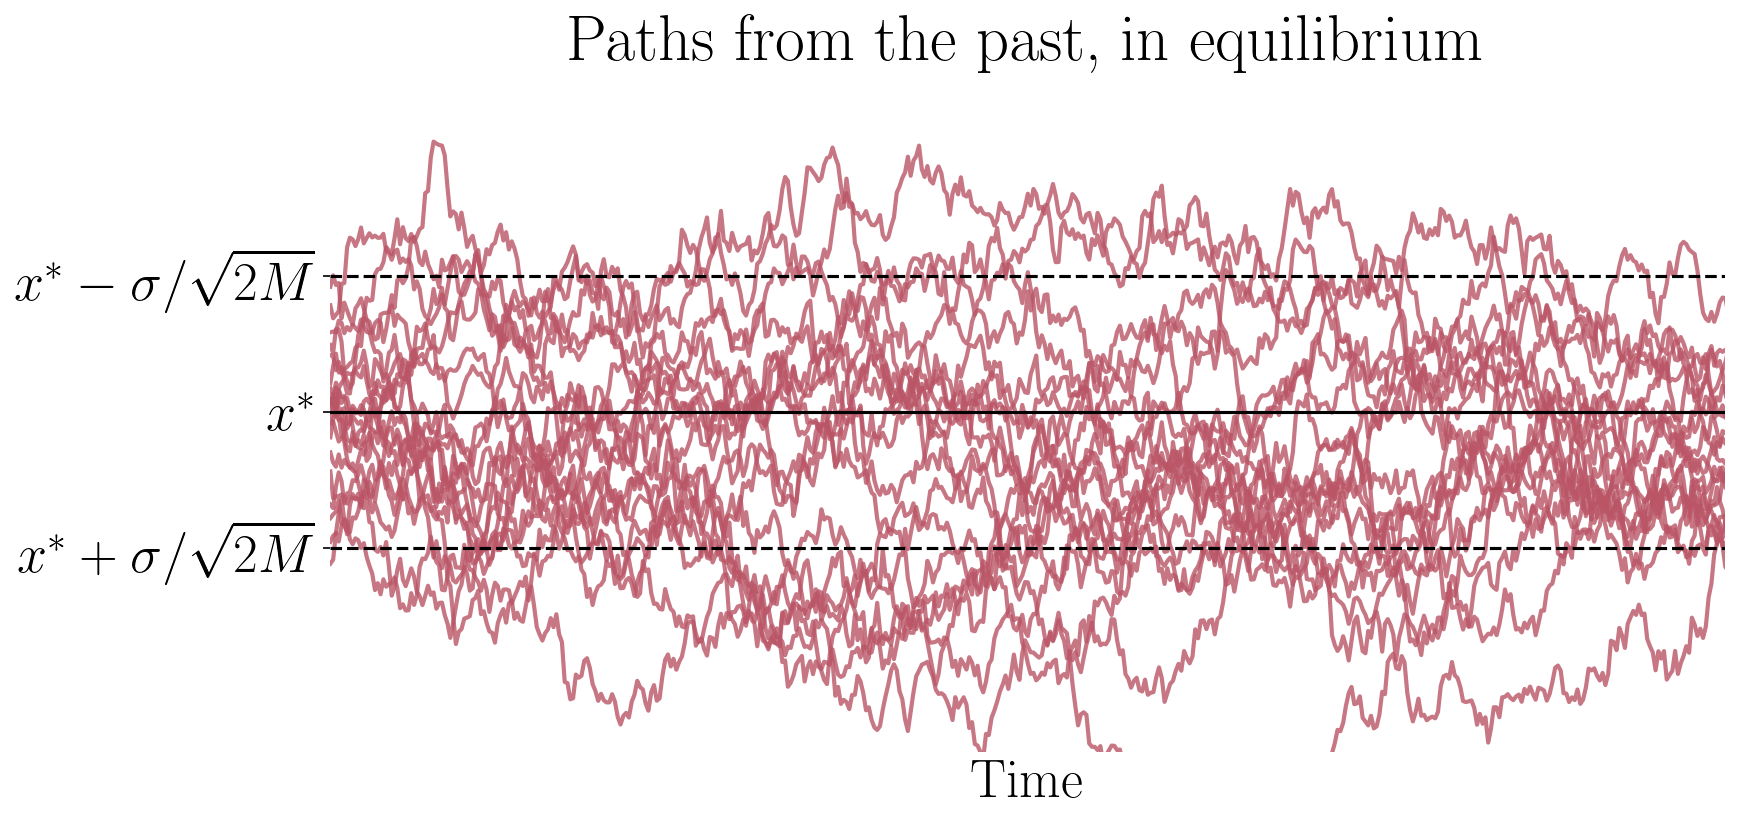
\includegraphics[width=0.9\linewidth]{Images/Metrics/diff_init2}\\
	\caption{ Example of 20 integrations of \cref{eq: simplecase} with $\la=2$ and $c_\la=0$, where the initial condition are sampled from the expected equilibrium balance.}
	\label{fig:diffinit}
\end{figure}

Figure \ref{fig:diffinit} shows an example of 25 evolutions of \cref{eq: simplecase} with $\la=2$ and $c_\la=0$, assuming the initial condition come from  a far past so they are sampled from the expected equilibrium variance in \cref{eq: ST_variancelim}. 

\begin{figure}[tbp]
	\centering
	\includegraphics[width=\linewidth]{"../Programing Proyects/EE indicators/Simulations with pdfs to test/Stochastic equations/SDE tests jupyter/image_variance_speed/Good_test/toghether/000_variance_test_speed_toghether"}
	\caption{Comparison between the expected variance and mean, to the measured ones, both for an ensemble of 300 trajectories (orange) and for a single trajectory (blue). Theoretical expected values are shown in dashed black lines, the vertical red line marks the adiabatic threshold as defined in \cref{eq:noiseadiab} and the gray line marks the bifurcation point. This example shows sweeping rate $c_{\la}=2$ resulting in a fast sweeping region for $\la=[0,2.8]$.}
	\label{fig:000variancetestspeedtoghether}
\end{figure}


To test our hypothesis of using the criteria of \cref{eq:noiseadiab} as the limit to consider a slow sweeping of the parameter, we realize 300 integrations starting from initial conditions as shown in \cref{fig:diffinit} and we evolve the system from $\la_0=3$ to $\la_f=0.001$
 at different speeds, and calculate for each speed the variance and the mean for the ensemble of trajectories, and also for a  singular trajectory.
 
 Figure \ref{fig:000variancetestspeedtoghether} shows in orange the variance and the mean calculated from the ensemble values after a nonparametric block bootstraping after 500 bootstraps and using 70\% of the data length for each bootstrap. The values for calculated by bootstrapping the single trajectory are shown in blue.
 The top plot shows the variance and the expected equilibrium variance from  \cref{eq: ST_variancelim} in dashed black line.
 The middle lot shows the variance normalized to the expected  equilibrium variance from \cref{eq: ST_variancelim} to make more evident the deviation from the equilibrium.
 The bottom plot shows the mean, which is expected to be $0$, and in gray shows an example of a single raw trajectory.
 The vertical red line indicate the threshold defined by \cref{eq:noiseadiab}.
 This example shows sweeping rate $c_{\la}=2$ resulting in a fast sweeping region for $\la=[0,2.8]$
 
\begin{figure}[tbp]
	\centering
	\includegraphics[width=1\linewidth]{"../Programing Proyects/EE indicators/Simulations with pdfs to test/Stochastic equations/SDE tests jupyter/image_variance_speed/Good_test/toghether/014_variance_test_speed_toghether"}
	\caption{Same analysis as in \cref{fig:000variancetestspeedtoghether}. This example shows a slower sweeping rate $c_{\la}=0.0074$ resulting in a fast sweeping region for $\la=[0,0.2]$.}
	\label{fig:014variancetestspeedtoghether}
\end{figure}


Figure \ref{fig:014variancetestspeedtoghether} shows the same information, for a slower sweeping were in can be seen that ensemble and single trajectory statistics behave similarly until close to the to the adiabatic threshold in with  \ref{fig:000variancetestspeedtoghether}.

From this test we can see that   \cref{eq:noiseadiab} in this particular case predicts qualitatively when the ensemble statistics deviate from the expected values.
Therefore the sweeping speed is clearly relevant even in cases when the system trivially close tracks $x^*$.

For completeness, in \cref{fig:stats} we analyze the EWS of interest for the case where  we don't sweep the control parameter but we evolve it by steps. That is, we analyze each case for a constant value of $\la$, then we move to the next value $\la-\Delta \la$ using the last value as initial condition, waiting for a transient time, and we re-do the analysis. 
To increase the resolution near the bifurcation, the values of $\la$ are logarithmically spaced between $\la_0=3$ (check) and $\la_f=0.001$. 

Each point the is result of calculating the EWS by bootstraping like in the previous case, for an original sample of 3690 point.
\begin{figure}
	\centering
	\includegraphics[width=0.9\linewidth]{"../Programing Proyects/EE indicators/Simulations with pdfs to test/Stochastic equations/SDE tests jupyter/image_variance_speed/skipping/stats"}
	\caption{Analysis of the EWS for the autonomous case of \cref{eq: simplecase} with a stepped evolution of $\la$. To increase the resolution near the bifurcation, the values of $\la$ are logarithmically spaced.  }
	\label{fig:stats}
\end{figure}


In appendix \ref{apx:sameinit} we show the same analysis for the case where the initial conditions of the ensemble are all the same, thus keeping the information of the 'past'. In this case \cref{eq:noiseadiab} also marks a reasonable timescale for the memory of the system.



\section{Tracking timescale, and loss of symmetry in the augmented system}

It should be noted that, when investigating the ASS system, autonomous systems that are equivalent (same normal form), are not equivalent anymore. 

To exemplify this, we can look the transcritical bifurcation from the system
\begin{equation}
	\begin{cases}
		dx & = x(x-\la)dt+\sigma dW\\
		d\la & =c_\la dt
	\end{cases}
	\label{eq: tranc}
\end{equation}
whose non-autonomous equilibria are defined as $x^*=\left\lbrace 0,\la\right\rbrace $, with a bifurcation at $\la=0$ where the equilibria change stability. The LDR for the stable equilibria in this system is always $M=\la$.

We could do a translation of this system as  
\begin{equation}
	\begin{cases}
		dx & = (x-\la)(x-2\la)dt+\sigma dW\\
		d\la & =c_\la dt
	\end{cases}
\label{eq: tranc_sl}
\end{equation}
now the deterministic autonomous backbone of this systems are the same, except that the equilibria are translated by $\la$, $x^*=\left\lbrace \la,2\la\right\rbrace $; and $M=\la$ for all the stable equilibria. 

However, for \cref{eq: tranc}, the stable equilibria $x^*={0}$ has not rate-dependence, furthermore, after it turns unstable it continues along the same path as $x^*_u={0}$. 
If we look at what happens to the ASS system (\cref{fig:transcr}), with $c_\la=0.02$ and $\sigma=0.01$, the paths generated from sweeping $\la$ from positive to negative (red) have an equal chance of diverging or going to the new equilibrium. 
While the  paths generated from sweeping $\la$ from negative to positive (yellow) are all will not diverge since the deviation due to the rate keeps them completely contained on the basin of the stable equilibrium.  

\begin{figure}[htb]
	\centering
	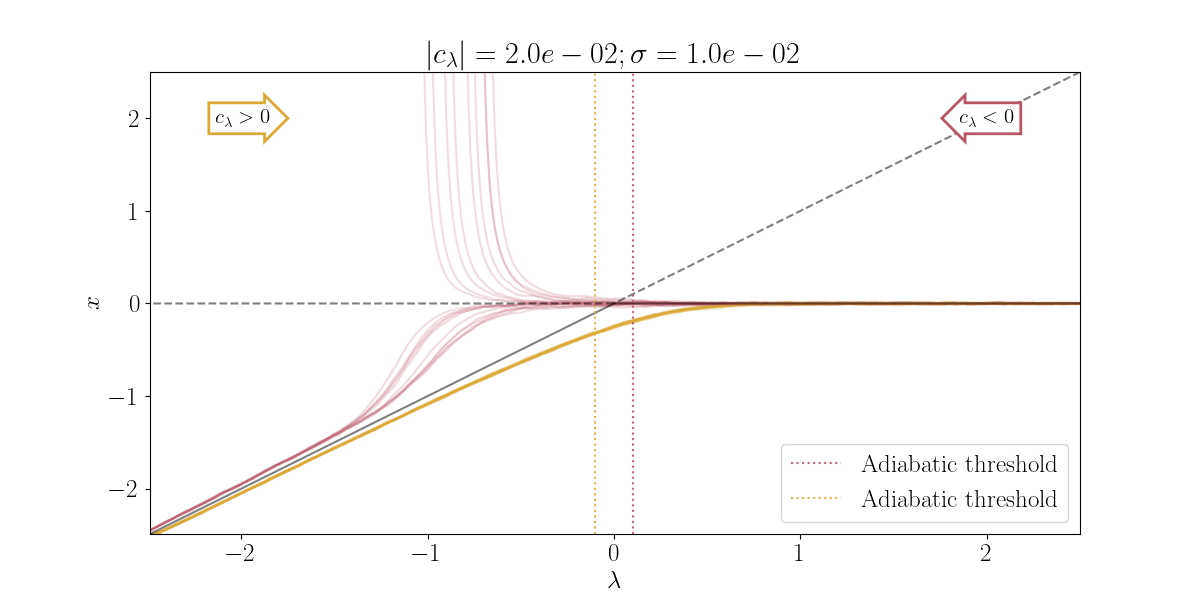
\includegraphics[width=\linewidth]{Images/Metrics/nonnormality/transcr}
	\caption{Integration of 20 different paths of \cref{eq: tranc} sweeping from negative to positive $\la$ (yellow) and vice-versa (red), with $c_\la=0.02$ and $\sigma=0.01$. Vertical dotted lines identify the adiabatic limit from \cref{eq:noiseadiab} for the respective branches. }
	\label{fig:transcr}
\end{figure}

If we look to what happens to \cref{eq: tranc_sl}, for the same sweeping speed and the same noise, all the trajectories in the positive to negative sweep diverge, and do so faster than in the previous case. 

\begin{figure}[htb]
	\centering
	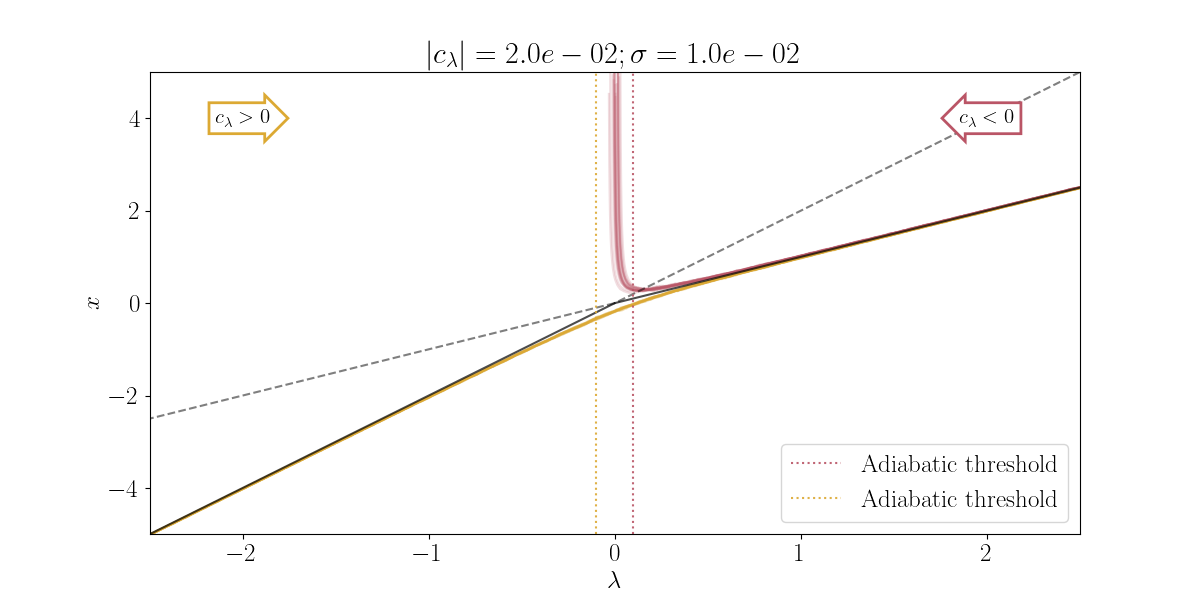
\includegraphics[width=\linewidth]{Images/Metrics/nonnormality/transcr_sla}
	\caption{Integration of 20 different paths of \cref{eq: tranc_sl} sweeping from negative to positive $\la$ (yellow) and vice-versa (red), with $c_\la=0.02$ and $\sigma=0.01$.  Vertical dotted lines identify the adiabatic limit from \cref{eq:noiseadiab} for the respective branches.}
	\label{fig:transcrsla}
\end{figure}

Now there is also a deviation due to the rate of sweeping in the other branch, and all the trajectories get pushed towards the unstable basin before the bifurcation happens. 

The difference in tipping time in this case is also affected by the rate. 
In \cref{fig:transcr}, near after the bifurcation, the systems stays doing a Brownian motion around the unstable equilibria, and since the local potential landscape is very flat $M\approx 0$ it will diverge once a the random walk takes it far away enough of the hill, and/or the hill becomes concave enough to repel the system.

While in \cref{fig:transcrsla}, even if the system does not completely tip before the bifurcation, the divergence of the trajectory will be faster as in this case the system cannot do a random walk in the unstable equilibrium after the bifurcation since the equilibrium itself moves away. 

We add in appendix \ref{apx:simetrictranscrit} a full symmetric case as a further example, plus a similar example for the normal form of a subcritical pitchfork bifurcation and a translated version.

This effect can have important implications in the reversibility of a system after a bifurcation. If we consider a system that evolved slowly from negative to positive values of the control parameter, when trying to recover the system to the old behavior, retracting fast is worst that retracting slow and the system might tip before showing signs of slowing down. 

\begin{figure}[htb]
	\centering
	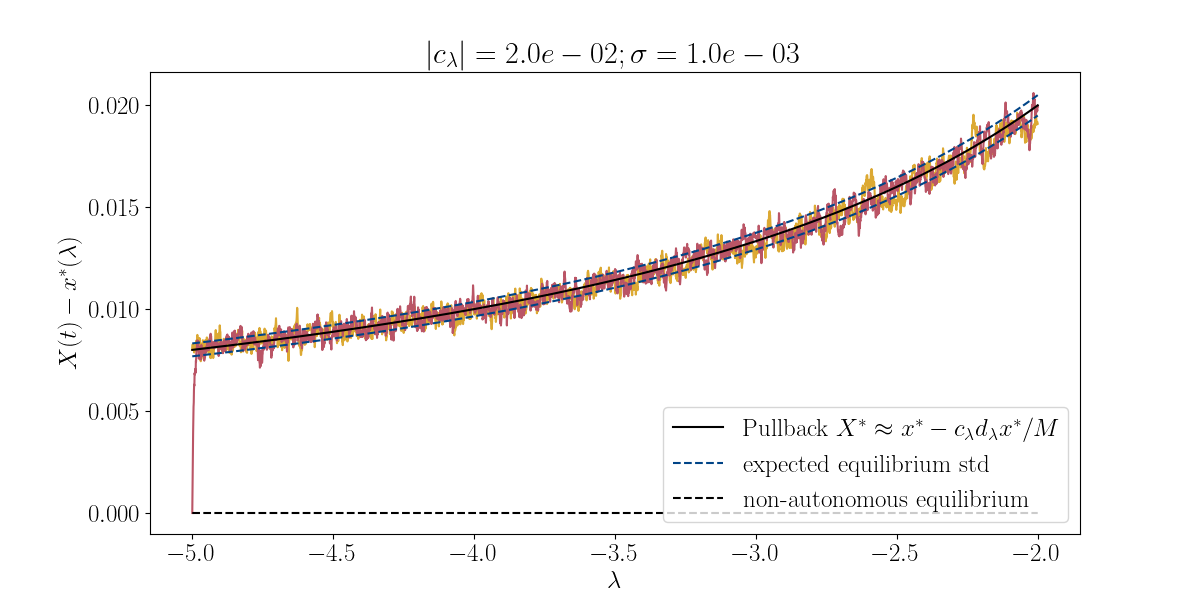
\includegraphics[width=1\linewidth]{Images/Metrics/nonnormality/deviation_trancr}
	\caption{Example of close tracking on \cref{eq: tranc_sl} for a slow variation of the control parameter. The dashed line represents the stable equilibrium ($x^*$) which is set to zero for plotting purposes. Two trajectories are displayed. The red has an initial condition at $x^*$ while the yellow starts at the expected correction from the linear instantaneous lag. The solid black line is the expected path from the linear correction and the dashed lines are the expected standard deviation from \cref{eq: ST_variancelim}. }
	\label{fig:deviationtrancr}
\end{figure}

Inspired by the results of \cref{eq:noiseadiab} we propose
\begin{equation}
		\tcbhighmath{
	t_{\mathrm{sweep}}=\int \frac{d\lambda}{c_\lambda} 
}
\end{equation}
as a characteristic timescale for the sweeping parameter. I should be noted that the integral is not defined when $c_\la=0$ being consistent with not having a timescale if there is no sweeping.
So we propose to compare this timescale  to the relaxation timescale results in  
\begin{equation}
		\tcbhighmath{
	\int  \frac{d\la}{c_\la} > -\frac{1}{||M||}.}
\end{equation}
We will show that this timescale will define the range of validity of the approximation of the instantaneous lag and gives a clear definition for close tracking in terms of the control parameter speed and the attraction of the stable equilibrium. 
As a bonus, it also gives a regime on which the  effective tipping radius $R$ from \cref{eq:Ashwin_track} is approximately the same as the basin radius.

Using as example the negative stable branch of \cref{eq: tranc_sl}, \cref{fig:deviationtrancr} display the deviation from the expected linear instantaneous lag correction as a function of the sweeping rate $c_\lambda$, for the range where we still consider a slow sweeping. The dashed line is the detrended stable branch $x^*=2\la$, the solid black line is the expected deviation due to the instantaneous lag, surrounded by blue dashed lines showing the expected equilibrium standard deviation from \cref{eq: ST_variancelim}. The red trajectory has an initial condition on the $x^*$ branch while the yellow trajectory has an initial condition on the expected position due to the instantaneous lag.



Figure  \ref{fig:adiabrtipdef010} and \cref{fig:adiabrtipdef039} display the deviation from the expected linear instantaneous lag correction as a function of the sweeping rate $c_\lambda$ and the proximity to the bifurcation. 
Figure \ref{fig:adiabrtipdef010} shows a slower sweeping rate, where the system follows the expected variance and trajectory of the linear correction up to the dashed blue line, close to the bifurcation. 
The top plot shows the trajectory in red, the stable and unstable branches, the expected path as a  dashed-dotted line (which diverges at the bifurcation), the yellow dotted line shows the limit up to which we expect the system to close track ($\int d\la/c_\la =1/M$), and the blue line  is defined as a tighter restriction ($\int d\la/c_\la =10/M$).
The middle plot shows the same information, translated to $x^*$ for plotting purposes. 



The bottom plot shows in log scale the normalized (to the pullback attractor $X^*$) deviation from the linear instantaneous lag correction. 
Here we can see that the criteria ($\int d\la/c_\la =1/M$) matches an order 0 deviation from the expected value, while ($\int d\la/c_\la =10/M$) is gives a deviation between $1\%$ and $10\%$ of the expected value. 


\begin{figure}[htb]
	\centering
	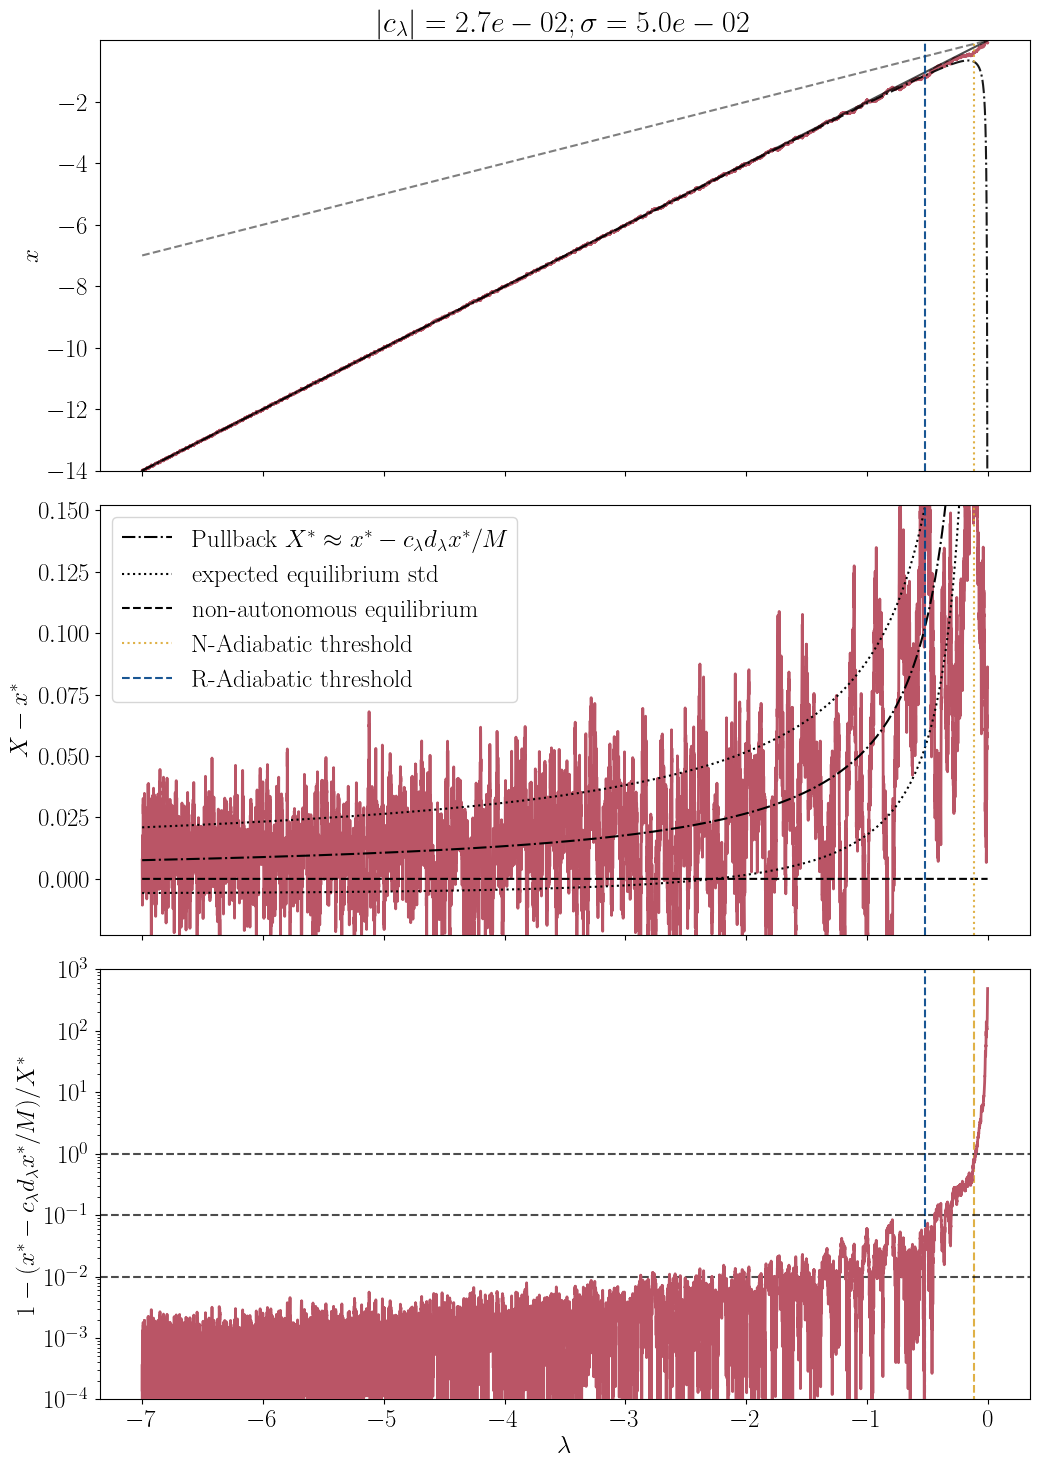
\includegraphics[width=0.9\linewidth]{Images/Metrics/traking/adiab_rtip_def010}
	\caption{Slower sweeping example.  }
	\label{fig:adiabrtipdef010}
\end{figure}

\cref{fig:adiabrtipdef039} shows a faster sweeping rate. In this case, the system deviates from the expected linear correction much faster. However as we can see from the bottom plot, the same features are retained, where the criteria ($\int d\la/c_\la =1/M$) matches an order 0 deviation from the expected value, while ($\int d\la/c_\la =10/M$) is gives a deviation between $1\%$ and $10\%$ of the expected value. 

\begin{figure}[htb]
	\centering
	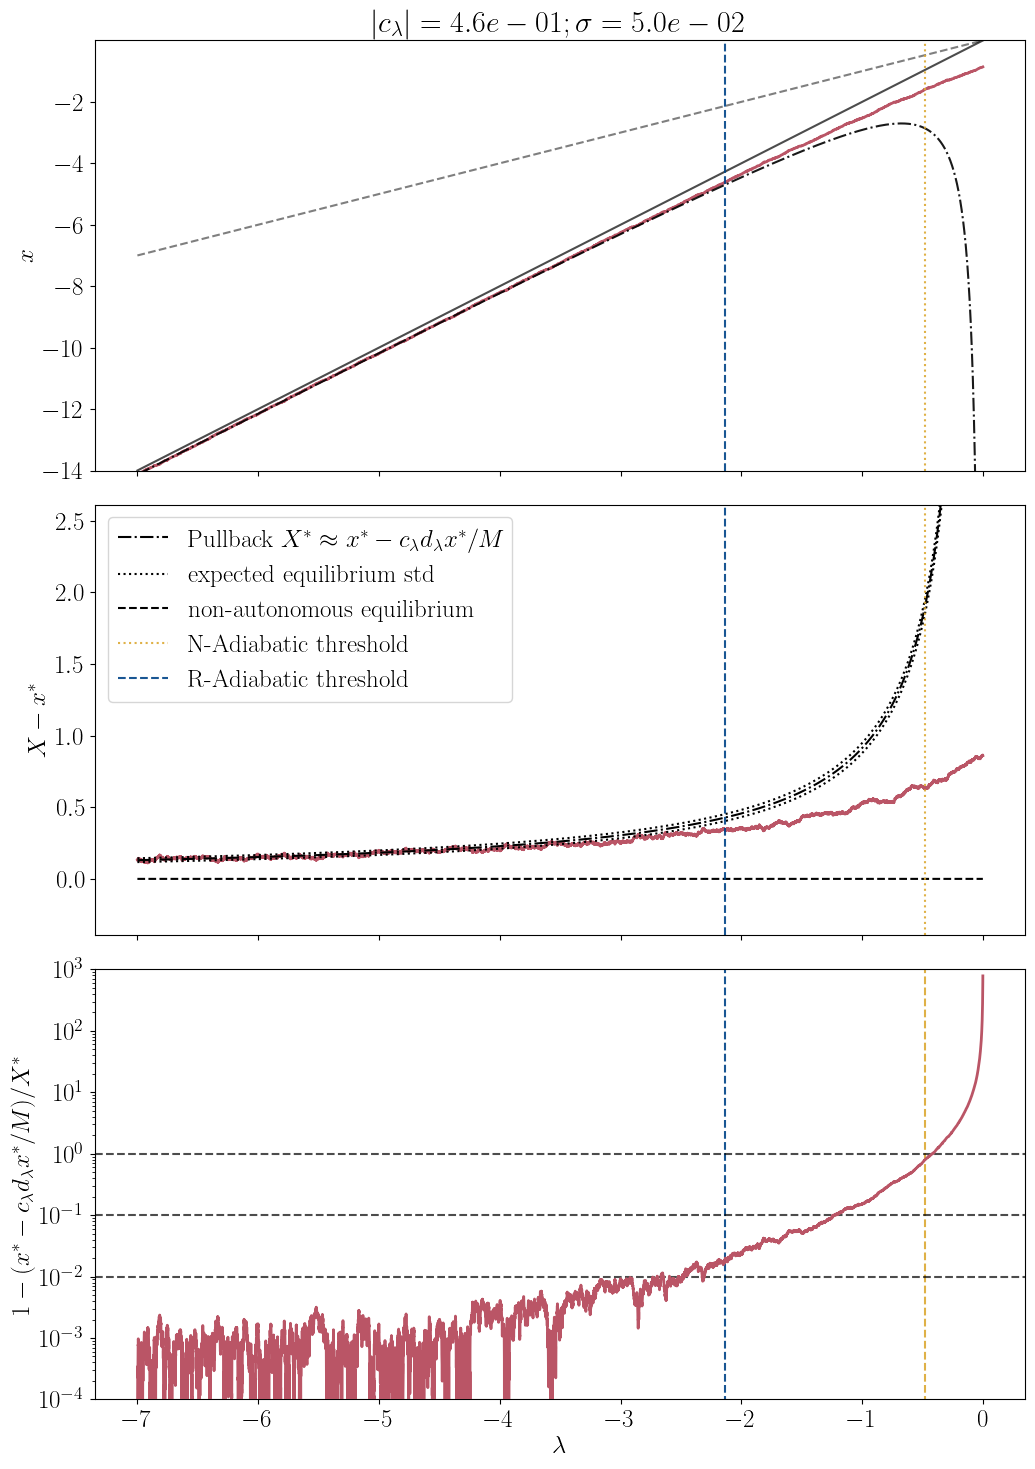
\includegraphics[width=0.9\linewidth]{Images/Metrics/traking/adiab_rtip_def039}
	\caption{Faster sweeping example.}
	\label{fig:adiabrtipdef039}
\end{figure}

Thus comparing the scale defined by $\int d\la/c_\la =1/M$ seems to give a reasonable scale to the define a threshold for slow variation in terms of close tracking, defined as the pullback attractor following the linear instantaneous lag.
This is also a reasonable definition for adiabatic sweeping since it relates to the definition for adiabatically in the stochastic sense ($\int d\la/c_\la =1/2M$)
and it is related to following a path calculated by assuming the $M$ does not change. 
In other words, this scale defines up to which point the control parameter changes slow enough that we might consider $M$ (or conversely, the return rate) at each point in time, the same as in the autonomous case. 
Again, close enough to the bifurcation this assumption will always fail. This adiabatic definitions define where (or when) is close enough for each sweeping speed. 


